
Well localized electron sources represent excellent calibration tool for the study of electron transport in the \dshort{lartpc}. 
%dword{lar} \dword{tpc}.
%, identification of the inhomogeneities in the TPC \efield in all directions, and precise determination of the electron drift velocity. Verification and calibration of the \efield distortions play an important role in particle vertex reconstruction and identification and affects the associated systematic errors, leading to increased rate of mis-identification and poorer energy reconstruction. 
%A photoelectron laser system can provide such sources at predetermined locations on the cathode, leading to precise  measurements of total drift time and of integrated spatial distortions (when the charge is not collected in the expected wires), and therefore to an improved characterization of the \efield, and consequent reduction of detector instrumentation systematic errors.
A photoelectron laser system can provide such sources at predetermined locations on the cathode, leading to precise  measurements of total drift time and integrated spatial distortions when the charge is not collected in the expected wires. These are achieved by simply measuring the time difference between the laser pulse trigger time and the time when the electron cloud reaches the anode plane assembly. Such measurement will result in an improved spatial characterization of the \efield, and consequent reduction of detector instrumentation systematic errors.

Being an operationally simpler system compared to the ionization laser system, the photoelectron laser can be used as a ``wake-up'' system to quickly diagnose if the detector is alive, and to provide indications of detector regions that may require a fine-grained check with the ionization system. This is especially important due to the low cosmic ray environment in the detector underground. The photoelectric laser system will utilize the ionization laser for target illumination, thus eliminating the additional cost associated with the laser purchase.


%
%leading to improved characterization of the \efield, and consequent reduction of detector instrumentation systematic errors. The photoeletron laser system, being a simpler system operationally compared to the ionization laser system, can be used as a wake-up system to quickly diagnose if the detector is alive. This is especially important due to the low cosmic ray environment in the detector underground. 

\subsubsection{Design}
\label{sec:sp-calib-sys-las-pe-des}

In order to produce localized clouds of electrons using a photoelectric effect, small metal discs will be placed on the cathode plane assembly and used as targets. Photoelectric laser systems have been successfully used at T2K~\cite{Abgrall:2010hi} and in the Brookhaven National Laboratory (BNL) \dword{lar} test-stand~\cite{Li:2016ods} to generate well-localized electron clouds for \efield calibration. 

%The baseline material choice for the metal targets is aluminum, while the alternatives such as silver, gold and nickel are under consideration. As stated in reference~\cite{Li:2016ods}, gold film can be just \SI{22}{\nano\m} thick. Thus the choice of metal will not significantly impact the overall cost of the targets. At \SI{266}{\nano\m} (Nd:YAG quadrupled wavelength) the single photon energy of \SI{4.66}{\eV} is sufficient to generate photoelectrons from aluminum and silver, but not from gold or nickel, that both have a higher work function than \SI{4.66}{\eV}. The solution in the case of gold and nickel is the use of the fifth harmonic of the Nd:YAG laser at \SI{213}{\nano\m} with energy of \SI{5.82}{\eV} which is above the work function of gold and nickel. The fifth harmonic can be added to standard Nd:YAG lasers as needed. The main advantage of gold film is that its surface is easier to protect from contamination, while aluminum, silver and nickel are prone to oxidization which changes their work function. In the case of aluminum, a thick layer of aluminum oxide forms the surface, but this does not increase the work function of the material. Table~\ref{tab:metalphotoelectric} lists the relevant features of metals under consideration.  

The baseline material choice for the metal targets is aluminum, while silver is being considered as an alternative. At \SI{266}{\nano\m} (Nd:YAG quadrupled wavelength) the single photon energy of \SI{4.66}{\eV} is sufficient to generate photoelectrons from aluminum and silver. However, aluminum and silver are prone to oxidization.
%which changes their work function. 
In the case of aluminum, a thick layer of aluminum oxide forms the surface, but this does not increase the work function of the material. Table~\ref{tab:metalphotoelectric} lists the relevant features of metals under consideration.  

The main factor driving the electron yield from the photoelectric targets is the quantum efficiency of the material. Although electrons will be released from the metal whenever photons hit the metal surface, most of the ejected electrons carry forward momentum and therefore are never released from the metal. Only a small fraction of released electrons back-scatters or knocks another electron out of the surface. The quantum efficiency for various metals is typically between \num{e-5}  and \num{e-6}, thus quite low.  All material candidates will be studied in the lab to verify the electron yield, and tested in \dword{protodune2} in order to verify the quantum efficiency for different materials.

\begin{dunetable}
[Work function and other features of candidate metal targets for laser photoelectron system]
{cccccc}
{tab:metalphotoelectric}
{Work function and other features of candidate metal targets for laser photoelectron system.}
 Target Material & Work function (\SI{}{\eV}) & $\lambda_{max}$ (\SI{}{\nano\m}) & $\lambda_{laser}$ & Oxidizing & Type of \\ 
\rowtitlestyle 
  & & & required (\SI{}{\nano\m}) & in air & oxidization \\ \toprowrule
 %Gold & 5.1 & 243 & 213 & No & None\\ \colhline
 %Nickel & 5.04 &  246 & 213 & Yes & Surface layer \\ \colhline
 Aluminum & 4.06 & 305 & 266 & Yes & Surface layer \\ \colhline
 Silver & 4.26-4.73 & 291 & 266 & Yes & Surface layer \\ 
  & (lattice dependent) & & & & \\ %\colhline
\end{dunetable}

%At S\I{266}{\nano\m} Nd:YAG quadrupled wavelength, the photon energy of\SI{4.66}{\eV} is sufficient to generate photoelectrons from both aluminum and gold. 

Disc targets will be fabricated with two different diameters: \SI{5}{\milli\m} and \SI{10}{\milli\m} to provide a test of the vertex reconstruction precision. In addition to circular targets, metal strips \num{0.5} $\times$ \SI{10}{\cm} are being considered to calibrate the rate of transverse diffusion in \dword{lar}. However, their impact on the cathode field will be carefully studied before being incorporated into target list, to prevent any disruptions to the cathode electric field.  

The targets will be fastened to field shaping strips located on the rim around the resistive panel of the cathode plane assembly. Figure~\ref{fig:calib-PhotoelectricTargets} illustrates locating the photoelectric targets on the rim around the resistive panel. The distance between the dots will be \SI{10}{\cm} with \num{5} targets at each corner, while the strips will be fastened at the center of each long side of the resistive plane. The total number of disc targets per resistive panel is \num{20} and the total number of strips per resistive panel is \num{2} as illustrated in Figure~\ref{fig:calib-TargetsOnCPA}.  Given that there are \num{600} resistive panels per \single module, there will be a total of \num{12000} disc targets and \num{1200} strip targets per module. %The final number of targets and their locations will be based on the calibration needs and simulation outcomes. 
The photoelectric dots and strips layout will be further refined based on the calibration requirements and performance simulation results. It will be essential to conduct a survey of the photocathode disc locations on the cathode after installation and prior to detector closing. In this way, the absolute spatial calibration of the \efield will be achieved. 

\begin{dunefigure}[Placement of phototargets on the cathode plane assembly]{fig:calib-PhotoelectricTargets}
{The best place to place the photo targets without being intrusive for the \efield, is the surface of the field shaping strips around the rim of the resistive panel. Circular targets will be implemented, while the strip targets are still under consideration.}
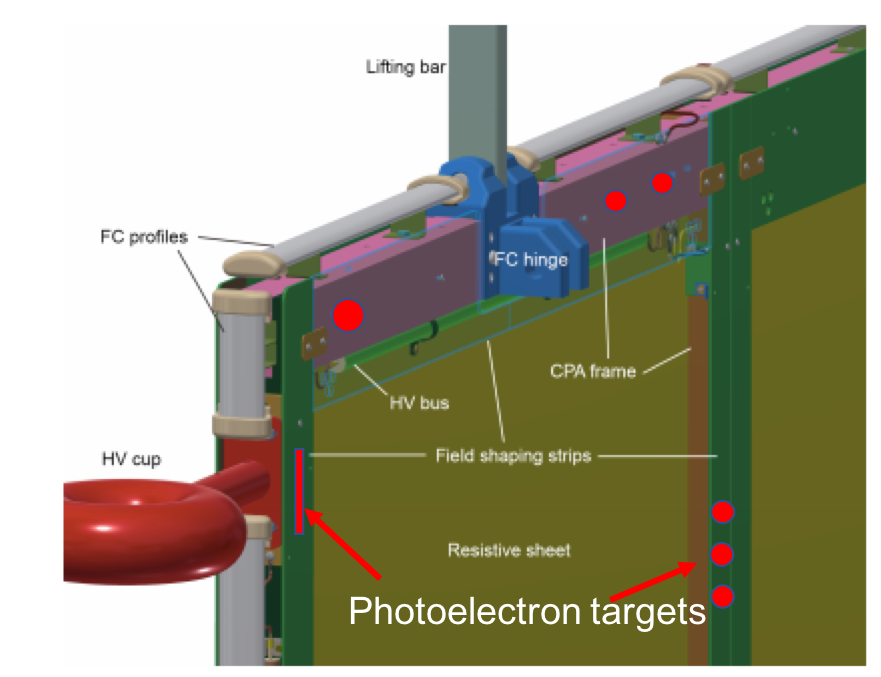
\includegraphics[width=0.65\linewidth]{calib-PhotoelectricTargets.png} 
%\label{fig:calib-PhotoelectricTargets}
\end{dunefigure}

\begin{dunefigure}[Anticipated positions and number of  phototargets on the cathode plane assembly]{fig:calib-TargetsOnCPA}
{There are a total of 5 circular targets in each corner, for a total of 20 circular targets: 12 large and 8 small diameter targets total. In addition, 2 strips at the center along the long sides of the resistive panels may be added if not disruptive to the high voltage on the cathode plane.} 
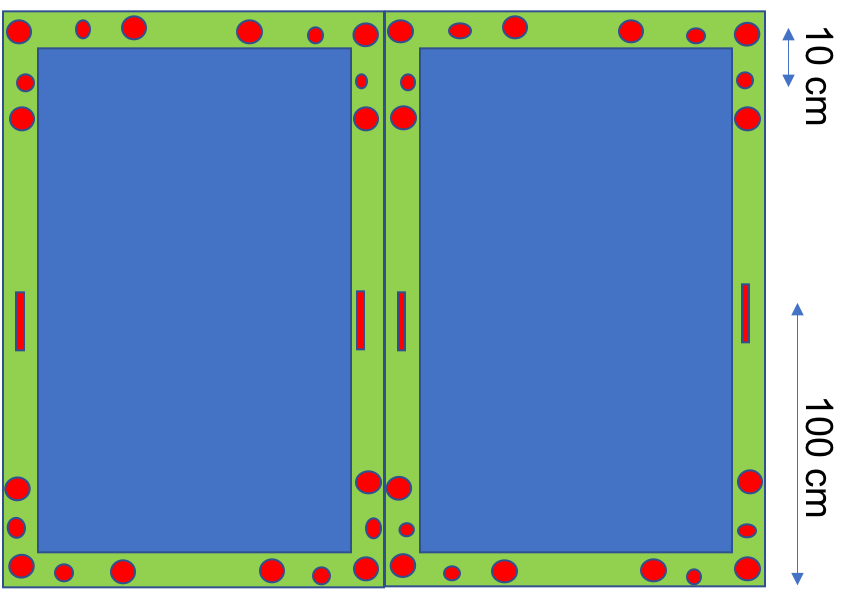
\includegraphics[width=0.55\linewidth]{calib-TargetsOnCPA.png} 
%\label{TargetsOnCPA}
\end{dunefigure}

A few thousand electrons are required per spill from each dot to produce the signal above the noise level on the wire and this number will be achieved with high intensity lasers (pulses of the order of \SI{100}{\milli\joule}). The laser beams used to illuminate the targets will be injected into the cryostat via cryogenic optical fibers guided into mounting points in the \dword{apa}, where they are coupled with defocusing elements that will illuminate \SI{10}{\m} diameter surface on the \dword{cpa}  with a single fiber. Fibers will be fastened along the central line of the \dword{apa} in the space between the top and bottom \dword{apa}, on the top of the upper \dword{apa} and on the bottom of the lower \dword{apa}. With the aid of the defocusing elements, the entire single phase module can be illuminated with a total of \num{72} fibers, corresponding to just \num{6} fibers along the central line along with \num{6} fibers on top and bottom for a total of \num{18} fibers per each of the four drift volumes. Figure~\ref{fig:calib-CPAIllumination} shows the conceptual view of the \dword{cpa} illumination.
%while Figure~\ref{fig:calib-TPCLaserInjection} shows the top of the cryostat with labeled tentative positions of the fiber injection. 

\begin{dunefigure}[View of the \dshort{cpa} illumination with fibers on the \dshort{apa}]{fig:calib-CPAIllumination}
{Conceptual view of the \dword{cpa} illumination with fibers placed on the top and bottom of the \dword{apa} for better coverage and overlap.} 
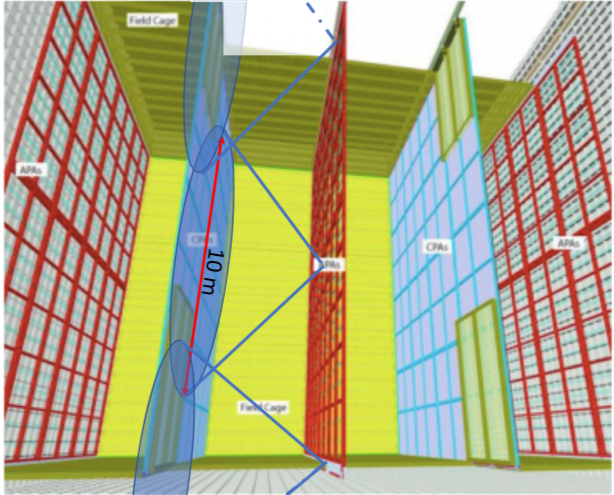
\includegraphics[width=0.55\linewidth]{calib-CPAIllumination.png} 
%\label{TargetsOnCPA}
\end{dunefigure}

%\begin{dunefigure}[Top view of the TPC with laser injection positions labeled in the figure. ]{fig:calib-TPCLaserInjection}
%{Locations of the laser injection points on the top of the cryostat.} 
%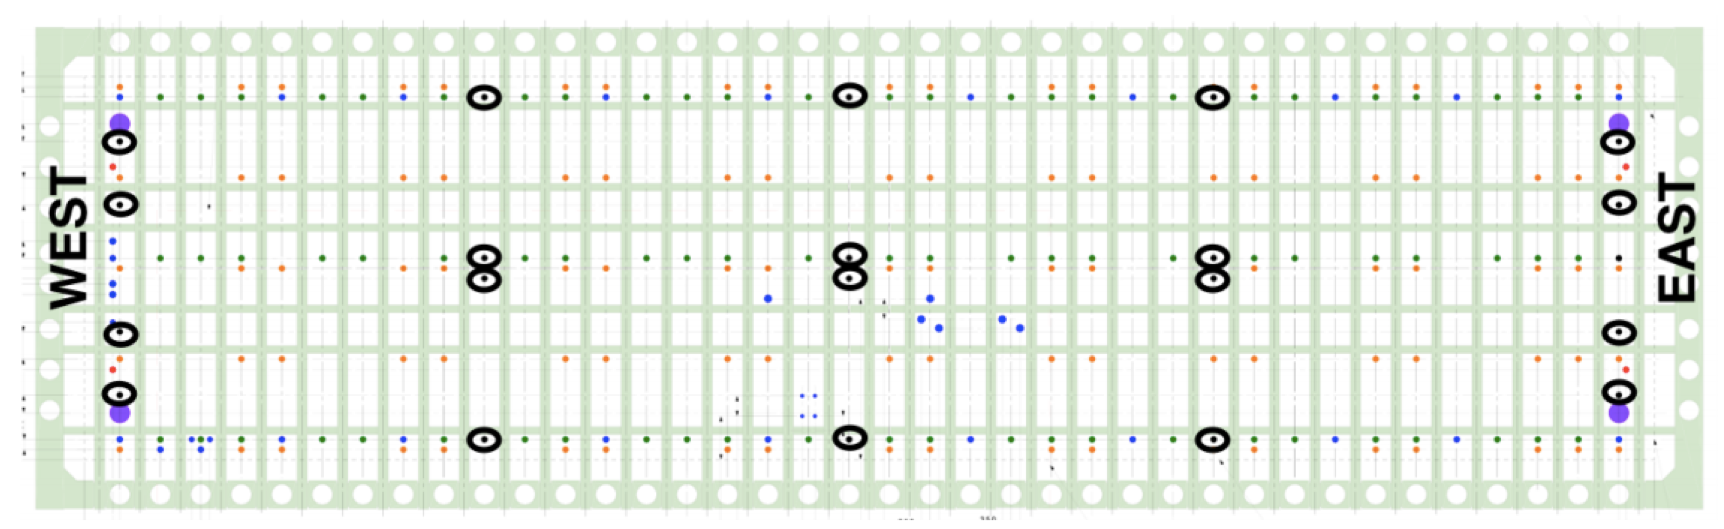
\includegraphics[width=0.8\linewidth]{graphics/calib-TPCLaserInjectionPoints.png} 
%\label{TargetsOnCPA}
%\end{dunefigure}

While the current plan aims for illumination of the entire \dword{cpa}, the Kapton material that composes the resistive panels undergoes photoelectric effect, albeit with three orders of magnitude lower quantum efficiency at cryogenic temperatures when compared to phototargets at \SI{266}{\nano\m}. While the noise produced is expected to be tolerable, in case the noise is higher than anticipated, the solution is to illuminate only the areas where phototargets are placed reducing the resistive panel exposure. In this case, instead of defocusing element, bare fibers will be utilized. The bare fiber opening angle is \ang{10} and \SI{1.3}{\m} diameter exposure.   
Assuming parallel running of lasers, photoelectron targets in 3 out of 4 volumes can be illuminated at once, assuming that laser firing can be coordinated and calibrated with sufficient precision and that volumes 2 and 3 share lasers. Lasers typically operate at 10 Hz frequency. If 10000 pulses per laser are assumed, about 15 minutes of running is needed per laser for a single calibration run
%, since 
as the photoelectron clouds from different dots are very well localized.
With the help of commercial multiplexers per each volume, 1 hour per volume will be sufficient for a single calibration campaign. If the \dword{daq} or lasers themselves prevent parallel running, the entire calibration campaign will take between 15 minutes or up to 1-5 hours. The calibration run duration will depend on the final calibration scheme.

The photoelectron system will use the same lasers used for argon ionization. Stability of the laser pulses will be monitored  with  a power meter. Dielectric mirrors reflective to \SI{266}{\nano\m} light will guide the laser light to injection points, but a fraction of the light will be transmitted instead of reflected to the power meter behind the mirror. The laser will also send a forced trigger signal to the \dword{daq} based on the photodiode that will be triggered on the fraction of the light passing through the dielectric mirror. 
%Special mirrors reflective to \SI{266}{\nano\m} light will be utilized. 

\subsubsection{Development plan}
The photoelectron system will require the following tasks to complete the design that can be done in \dword{protodune2} or in the lab: 
\begin{itemize}
    \item test the mounting of the targets on the \dword{cpa}
    \item use different target materials to compare their performance
    \item verify the potential of targets to generate several \SI{1000} electron clouds and their %potential 
    ability to diagnose electric field distortions and vertex reconstruction
    %\item search for noise related to photoelectron targets in the ProtoDUNE-II data
    %\item search for noise related to running the PhEL in the ProtoDUNE-II data from Kapton and other sources
    \item allocate ports to insert laser fibers used for illumination
    \item validate interface with %track 
    ionization laser in order to inject UV photons into fibers
    \item validate efficiency of laser light injection in the optical fiber
    \item validate light attenuation in fibers
    \item validate design interface with \dword{apa} and optimized locations of fibers between top and bottom \dword{apa}s  
    \item validate diffuser design and light losses in the diffuser as well as its ability to illuminate large areas of \dword{cpa}s
    \item validate bare fiber \dword{cpa} illumination
    \item survey of the dots position to the required level of precision; %and  
    %\item study thickness of the target and photoelectron yield as a function of target choice

\end{itemize}

\subsubsection{Measurement Program}
\label{sec:sp-calib-sys-las-pe-meas} 

Photoelectron systems have been used in other experiments to diagnose electronics issues by using the known time period between the triggered laser signal and read out times, and to perform rapid checks of the readout of the TPC itself. 

A photoelectron laser is an effective diagnostic and calibration tool, that can quickly and accurately sample the electron drift velocity in the entire detector.
In addition, it can be used to identify electric field distortions due to space charge effects. Exact knowledge of the timing and position of the generated electron clouds is useful for vertex calibration.
%The reciprocal of the \efield (integrated along the drift direction) is also measured.
In addition to electronics issues, discrepancies between the measured and expected drift time can point to either distortions in the position of the detector elements or to a different drift velocity magnitude. 

Another planned measurement is the comparison between the expected and measured $y$, $z$ position of the collected charge, that can point to transverse distortions of the \efield.




